\documentclass[letterpaper]{article}
\usepackage[utf8]{inputenc}
\usepackage[spanish]{babel}
\usepackage[letterpaper,includeheadfoot, top=.5cm, bottom=3.0cm, right=2.0cm, left=2.0cm]{geometry}
\renewcommand{\familydefault}{\sfdefault}
\usepackage{amsmath}
\usepackage{graphicx}
\usepackage{subcaption}
\usepackage{gensymb}
\usepackage{color}
\usepackage{hyperref}
\usepackage{amssymb}
\usepackage{url}
%\usepackage{pdfpages}
\usepackage{fancyhdr}
\usepackage{enumerate}
\usepackage{float}
\usepackage{tikz}
\usepackage{siunitx}
\usepackage{framed}
\tikzset{
every picture/.append style={
  execute at begin picture={\deactivatequoting},
  execute at end picture={\activatequoting}
  }
}
%-------------------- CABECERA ---------------------
\pagestyle{fancy}
\fancyhf{}
\author{Martin Bataille}
\date{}
\title{\bf Guía MCU}
%Encabezado
\fancyhead[R]{
\includegraphics[scale=0.35]{jct.jpg}}
\fancyfoot[C]{\thepage}


\newcommand{\tpb}[1]{node[midway, below, sloped] {#1}}
\newcommand{\tpa}[1]{node[midway, above, sloped] {#1}}
\newcommand{\tvec}[3]{[->, thick] #1 -- #2 \tpb{#3}}
\newcommand{\tveca}[3]{[->, thick] #1 -- #2 \tpa{#3}}
\newcommand{\tvecnotsloped}[3]{[->, thick] #1 -- #2 {node[midway, above] {#3}}}

\newcounter{propiedades}
\newcounter{definiciones}

\newcommand{\propi}{\stepcounter{propiedades} \textbf{Propiedad \thepropiedades}: }
\newcommand{\defii}{\stepcounter{definiciones} \textbf{Definición \thedefiniciones}: }

\newenvironment{prop}
{ \begin{framed} \propi}
{ \end{framed} }
\newenvironment{defi}{\begin{framed} \defii}{\end{framed}}

\renewcommand{\sectionmark}[1]{\markright{\thesection.\ #1}}
\renewcommand{\headrulewidth}{0.5pt}
\renewcommand{\footrulewidth}{0pt}
\setlength{\headheight}{92pt}

% --------------- ---------PORTADA -----------------------
\begin{document}
\maketitle
\thispagestyle{fancy}
\begin{center}
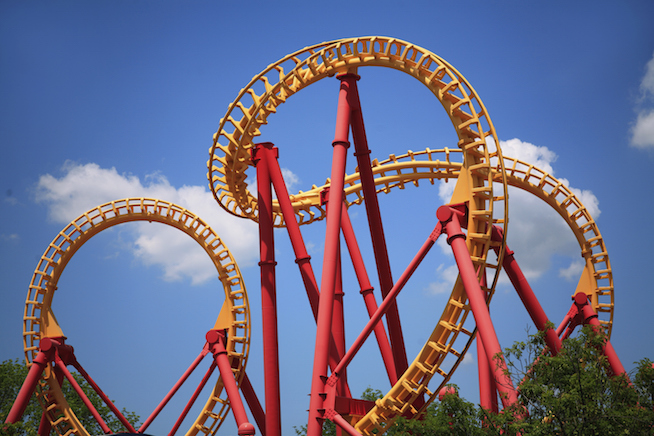
\includegraphics[scale=0.6]{portada.jpg}
\end{center}
\pagebreak

Cuando nos subimos a un montaña rusa y pasamos por un tramo circular, sentimos una "fuerza" que nos empuja al suelo, la famosa \emph{fuerza centrífuga}. Algunos podrían afirmar que es dicha fuerza la que evita que la Luna caiga a la Tierra y que permite que la Tierra siga su órbita en torno al Sol... Spoiler alert: ¡Esa fuerza no existe! Todo esto y mucho más lo explicaremos al estudiar este nuevo tipo de movimiento, el \emph{Movimiento Circular Uniforme} o \emph{MCU} para los amigos. 

\section*{¿Qué es el MCU?}

\begin{defi} 
Se dice que una partícula describe un movimiento circular uniforme cuando su trayectoria es circular y el módulo de la velocidad (la rapidez) es constante. Sin embargo, la velocidad como vector no es constante pues su sentido y dirección cambian en cada instante.
\end{defi}

\begin{figure}[h]
    \centering
    \begin{tikzpicture}
        \draw [dashed] (0,0) circle (2);
        \draw \tvec{(0,0)}{(10:2)}{$\vec{r}_1$};
        \draw \tvec{(0,0)}{(50:2)}{$\vec{r}_2$};
        \draw \tvec{(0,0)}{(90:2)}{$\vec{r}_3$};
        \draw \tveca{(30:2)}{++(120:2)}{$\vec{v}_1$};
        \draw \tveca{(70:2)}{++(160:2)}{$\vec{v}_2$}; 
    \end{tikzpicture}   
    \caption{Vectores posición y velocidad de una partícula en MCU.}
\end{figure}

En la figura anterior, podemos ver la posición de una partícula representada como un vector ($\vec{r}$) en 3 instantes distintos. Como ya sabemos, $$ \vec{v} = \frac{\Delta \vec{r}}{\Delta t} = \frac{\vec{r}_2 - \vec{r}_1}{t_2 - t_1} $$

Aplicando esta definición al caso anterior obtenemos dos vectores velocidad, $\vec{v}_1$ entre los instantes 1 y 2, y $\vec{v}_2$ entre los instantes 2 y 3. Podemos ver que el vector velocidad es perpendicular o \emph{tangencial} a la circunferencia, al menos en este caso. Esto siempre es cierto en todo movimiento circular (incluso si no es uniforme), el lector puede convencerse probando con distintos ángulos. 

\begin{prop}
En un movimiento circular el vector velocidad es siempre tangencial a la circunferencia que describe la partícula.
\end{prop} 

\textbf{Problema.} Nuestra amiga Camila está con su hermano menor Daniel en el Fantasilandia y se suben a una montaña rusa que termina en un tramo con forma de U, como en la figura. Justo antes de entrar a este último tramo, Camila ve que Daniel está muerto de miedo y le asegura que solo tendrá que aguantar 2 segundos más. ¿Es cierto lo que le dijo Camila? Asume que Camila y Daniel, representados por el punto en la figura, describen un MCU.

\pagebreak

\begin{figure}[h]
\centering
\begin{tikzpicture}
    \draw (-1, 2) -- (0,2) node {$\bullet$};
    \draw \tvecnotsloped{(0,2)}{(1,2)}{$\vec{v}_i = 18 \ \si{m.s^{-1}}$};
    \draw (-1, -2) -- (0,-2);
    \draw (0,-2) arc (-90:90:2);
    \draw [dashed] (0,-2) -- (0,2) node[left, midway] {$20\ \si{m}$};
\end{tikzpicture}
\caption{Diagrama del último tramo de la montaña rusa.}
\end{figure}

\section*{¿Cómo se describe un MCU?}

Para describir un MCU necesitaremos usar una nueva unidad de ángulo, el radian (\si{rad}).

\begin{defi}
 Se dice que un ángulo vale $\theta$ radianes cuando abarca un arco de circulo unitario de largo $\theta$.
\end{defi} 

Para visualizar un radian se puede dibujar un circulo de radio 1, también llamado circulo unitario. Un ángulo de $360\degree$ abarca toda la circunferencia por lo tanto, el arco abarcado vale $2\pi$ ya que el radio del circulo es uno. Entonces, por definición de radian, un ángulo de $360\degree$ equivale a un ángulo de $2\pi$ \si{rad}, así un ángulo de $180\degree$ equivale a $\pi$ \si{rad}. Digamos que queremos encontrar cuanto vale un ángulo de $60\degree$ en radianes.  
\begin{figure}[h]
\centering
\begin{tikzpicture}
\draw (0,0) circle (2);
\draw (0,0) -- (0:2) node[below, midway] {$1$};
\draw (-2,0) -- (0,0);
\draw (0,0) -- (60:2);
\draw (.9,0) arc (0:60:.9);
\draw (30:1.2) node {$\frac\pi3$};
\draw (.7,0) arc (0:180:.7);
\draw (0,.7) node[above] {$\pi$};
\end{tikzpicture}
\end{figure}

Basta con recordar que $60\degree = \frac{180}{3}\degree = \frac{\pi}{3}\ \si{rad}$. Es recomendable que el lector intente convertir los ángulos típicos ($30\degree$, $45\degree$, $90\degree$) en radianes.

\pagebreak

Podemos ahora definir unos cuantos conceptos que nos ayudarán a describir un MCU.

\begin{defi}
 La rapidez angular $\omega$, en radianes por segundo (\si{rad.s^{-1}}) de acuerdo al Système International d'Unités (SI), representa el cambio del ángulo en el tiempo, es decir, $$ \omega = \frac{\Delta \theta}{\Delta t} = \frac{\theta_2 - \theta_1}{t_2 - t_1} $$ 

 También es importante saber que existe la velocidad angular como vector, $\vec{\omega}$, el sentido y la dirección de la velocidad angular se determinan con la regla de la mano derecha: la dirección es siempre perpendicular al plano y, si el movimiento es en el sentido antihorario en el plano, el vector sale del plano, y en caso contrario, el vector entra al plano.
\end{defi} 

\begin{defi}
 El periodo $T$, en segundos de acuerdo al SI, representa el tiempo que le toma a la partícula en dar una vuelta completa a la circunferencia. Si una partícula describe un MCU a una velocidad de $\omega$ \si{rad.s^{-1}}. Sabemos que en recorrer un ángulo de $2\pi$ \si{rad} se demora $T$ segundos, es decir, $\omega = \frac{2\pi}{T}$. En otras palabras, $$T = \frac{2\pi}{\omega}$$
\end{defi}  

Es importante notar que si se demora $T$ segundos en recorrer una distancia de $2\pi r$, entonces $$|\vec{v}| = \frac{2\pi r}{T} = \frac{2\pi}{T} \cdot r = \omega r$$

De aquí podemos deducir una de las propiedades más importantes del MCU,

\begin{prop}
La velocidad tangencial y la velocidad angular están íntimamente relacionadas: $$|\vec{v}| = \omega r$$
\end{prop}

\begin{defi}
 La frecuencia $f$, en hertz ($\si{Hz} = \si{s^{-1}}$) de acuerdo al SI, representa la cantidad de vueltas que da la partícula en un segundo. Si una partícula se demora $T$ segundos en hacer una vuelta, entonces en un segundo hace $\frac{1}{T}$ vueltas, o sea, $$f = \frac{1}{T}$$
 \end{defi} 

\textbf{Ejemplo.} Si una partícula describe un MCU con una velocidad angular de $4\pi$ \si{rad.s^{-1}} entonces da dos vueltas en un segundo. El periodo es entonces $T = \frac{2\pi}{4\pi} = 0.5$ \si{s} y la frecuencia es $f = \frac{1}{T} = 2\ \si{Hz}$  

\vspace{1cm}

Volviendo al problema de Camila y Daniel sabemos que $\omega = \frac{|\vec{v}|}{r} = 1.8$ \si{rad.s^{-1}}. Por lo tanto, en recorrer medio circulo o $\pi$ \si{rad} Camila se demora $t = \frac{\pi}{1.8} \approx \frac{3.14}{1.8} < 2$. ¡Camila tenia razón! 

\section*{Momento de acelerar las cosas}

En un movimiento rectilíneo uniforme, la velocidad es constante, por lo tanto no hay aceleración. Sin embargo, en un movimiento circular uniforme, a pesar de que la rapidez es constante, existe una aceleración.

\begin{figure}[h]
\centering
\begin{tikzpicture}
 \draw [dashed] (0,0) circle (2);
 \draw \tveca{(60:2)}{++(150:1.5)}{$\vec{v}_1$};
 \draw \tveca{(90:2)}{++(180:1.5)}{$\vec{v}_2$};
 \draw \tveca{(120:2)}{++(210:1.5)}{$\vec{v}_3$};
 \draw [->, thick] (75:2) -- (75:0.5) {node[midway, right] {$\vec{a}_1$}};
 \draw [->, thick] (105:2) -- (105:0.5) {node[midway, left] {$\vec{a}_2$}};
\end{tikzpicture}
\caption{Vectores velocidad y aceleración en un MCU.}
\end{figure}

En la figura anterior, podemos ver los vectores velocidad en 3 instantes para un MCU, como ya sabemos,
$$ \vec{a} = \frac{\Delta\vec{v}}{\Delta t} = \frac{\vec{v}_2 - \vec{v}_1}{t_2 - t_1}$$


Aplicando esta definición obtenemos dos vectores aceleración que, curiosamente, apuntan hacia el centro de circulo. Si la aceleración no fuera perpendicular a la velocidad, entonces la magnitud de la velocidad cambiaría, por lo tanto, no sería un MCU. Es por esto que la aceleración es \emph{siempre} perpendicular a la velocidad y apunta hacia el centro de la circunferencia, uno habla entonces de aceleración centrípeta. Además, sabemos que,

$$
\vec{a} = \frac{\Delta \vec{v}}{\Delta t} = \frac{\Delta (\vec{\omega}\times\vec{r})}{\Delta t} 
= \vec{\omega}\times\frac{\Delta \vec{r}}{\Delta t} = \vec{\omega} \times \vec{v}
$$

En particular como el vector velocidad angular (que sale del plano de movimiento) es perpendicular al vector velocidad, 

$$|\vec{a}| = |\vec{\omega} \times \vec{v}| = \omega v = \omega (\omega r) = \omega^2 r = \frac{v^2}{r}$$

\begin{prop}
En todo MCU existe una aceleración hacia el centro de la circunferencia descrita por la partícula, se le llama aceleración centrípeta, se escribe $a_c$ y su magnitud está dada por,
$$ |\vec{a}_c| = \frac{|\vec{v}|^2}{r} = \omega^2 r $$
\end{prop}

\section*{Correas de Transmisión}

Una simple aplicación de un MCU que aparece en nuestra vida cotidiana son las correas de transmisión. Las bicicletas, por ejemplo, funcionan con este sistema que permite transmitir el movimiento del pedal a la rueda trasera, como lo muestra la figura.

\begin{figure}[h]
\centering
\begin{tikzpicture}
    \draw (0,0) circle (0.8);
    \draw (0,0) node {$\bullet$};
    \draw (5,0) node {$\bullet$};
    \draw (5,0) circle (1.6);
    \draw (0,0) -- (0.8,0) node[above, midway] {$r_1$};
    \draw (5,0) -- (6.6,0) node[above, midway] {$r_2$};
    \draw (94.11:0.8) -- (18.58:4.89);
    \draw (-94.11:0.8) -- (-18.58:4.89);
    \draw (5,0) -- ++(55:2.5);
    \draw [very thick] (5,0) ++(55:2.5) -- ++(0:0.5);
    \draw (5,0) -- ++(235:2.5);
    \draw [very thick] (5,0) ++ (235:2.5) -- ++(180:0.5); 
\end{tikzpicture}
\caption{Diagrama simplificado del funcionamiento de una bicicleta.}
\end{figure}

El empujar el pedal con el pie, se mueve el plato del pedal, representado como un circulo de radio $r_2$, al moverse el plato del pedal, se mueve el piñón de la rueda trasera, representado como un circulo de radio $r_1$, que provoca que la rueda trasera se mueva. Cuando el plato del pedal da una vuelta completa ($2\pi$ \si{rad}), la cadena de la bicicleta se mueve $2\pi r_2$ provocando que el piñón de la rueda trasera se mueva un ángulo de $2\pi\frac{r_2}{r_1}$ \si{rad}. Si $r_2$ es mucho mayor que $r_1$, digamos que $r_2$ es 5 veces más grande que $r_1$, entonces cuando el plato del pedal da una vuelta completa... ¡La rueda trasera da 5 vueltas!

\begin{prop}
 Sean $\vec{v}_1, \vec{v}_2$ y $\omega_1, \omega_2$ las velocidades tangenciales y angulares, respectivamente, de dos ruedas de radios $r_1, r_2$ respectivamente, unidas por una correa de transmisión, se tiene que
 
 \begin{equation*}
|\vec{v}_1| = |\vec{v}_2|\ , \qquad \omega_1 r_1 = \omega_2 r_2\ , \qquad \frac{\omega_1}{r_2} = \frac{\omega_2}{r_1}
 \end{equation*}
 
\end{prop}

\vspace{.5cm}

\textbf{Ejemplo.} Volviendo al funcionamiento de la bicicleta, al aplicar la propiedad anterior se tiene que la velocidad angular del piñón de la rueda trasera está dada por $$\frac{\omega_{pi\tilde{n}on}}{r_{pedal}} = \frac{\omega_{pedal}}{r_{pi\tilde{n}on}}, \qquad \omega_{pi\tilde{n}on} = \omega_{pedal}\frac{r_{pedal}}{r_{pi\tilde{n}on}}$$


De manera que si el radio del pedal es $5$ veces el del piñón, entonces la velocidad angular del piñón es $5$ veces la de la rueda y como el piñón está pegado a la rueda trasera, la velocidad angular del piñón es la misma que la de la rueda, por lo tanto, la velocidad angular de la rueda es $5$ veces la del pedal. 

\vspace{.5cm}

\textbf{Problema.} Nuestro amigo Daniel luego de salir del Fantasilandia, se propuso hacerle una carrera a su hermana, Camila. Claro que como Camila es más grande y rápida que Daniel, él agarró su bici y partió a toda velocidad, pedaleando a una velocidad angular $\omega = 6$ \si{rad.s^{-1}}, mientras que Camila salió detrás de él corriendo a toda velocidad. ¿Quién ganará la carrera? Asuma que Camila puede correr uniformemente a $15$ \si{km.h^{-1}} y que la bici de Daniel es tal que el radio del plato de los pedales es $12$ \si{cm}, el radio del piñón es $6$ \si{cm} y que el radio de la rueda de la bici es de $30$ \si{cm}.

\section*{Actividad paranormal: Fuerza centrífuga}

Probablemente una de las fuerzas más famosas es la que nos bota de las micros cuando giran muy rápido, la que nos permite secar la ropa en la secadora o la que nos empuja hacia afuera en una montaña rusa, así es: la fuerza centrífuga. Paradójicamente, ¡esta fuerza no existe! En física se le llama a este tipo de fuerzas, \emph{fuerzas virtuales} ya que no existen pero aún así se sienten como fuerzas. ¿Cómo se explica esto?


Para comprender el tema tenemos que saber lo que es un sistema inercial. Cuando vimos las leyes de Newton, la verdad es que esas leyes vienen con una letra chica: solo se aplican en un sistema inercial. ¿Qué es un sistema inercial? Pues un sistema en el que se aplican las leyes de Newton. De aquí surge una muy buena pregunta, ¿existe un sistema en donde no se cumplan las leyes de Newton? 

Podemos pensar en el metro, si dejas una maleta con ruedas en reposo en la mitad del metro, las únicas fuerzas que se aplican sobre la maleta son las fuerzas peso, normal, roce estático con el suelo (despreciable porque tiene ruedas) y roce con el aire (también despreciable). Sin embargo, sabemos que la maleta no se mueve verticalmente, por lo tanto, necesariamente la fuerza de peso es igual a la normal, mientras que en el eje horizontal no existe ninguna fuerza, o sea que, por la primera ley de newton, la maleta va a seguir en reposo. En la realidad, cuando el metro comienza a acelerar, la maleta se va al otro extremo del metro ya que se mantiene en reposo respecto a la estación de metro, no al metro en sí. El metro es entonces un sistema no inercial, ya que les las leyes de Newton no se cumplen, mientras que la estación de metro es un sistema inercial.

De manera general, un sistema es no inercial si acelera o rota con respecto a un sistema inercial. En el caso del metro, podemos pensar en la estación de metro como un sistema inercial ya que, efectivamente, las leyes de Newton se cumplen en la estación de metro, y, puesto que el metro está acelerando con respecto a la estación, el metro deja de ser un sistema inercial. Para poder aplicar las leyes de Newton en un sistema no inercial, hay que agregar fuerzas \emph{ficticias} o \emph{virtuales}, como la fuerza centrífuga. De esta manera, para estudiar el movimiento de la maleta, hay que introducir una fuerza ficticia que sería la responsable de que la maleta se escape al otro extremo del metro.                                                                                                                                   
\section*{Ejercicios}

Pendiente

\section*{Problemas}

\begin{enumerate}

\item Se está construyendo una nueva montaña rusa en Fantasilandia y hay una sección de la montaña rusa que se desea que sea en forma de \emph{loop}, ver figura siguiente. El equipo de diseño de montañas rusas de Fantasilandia quiere que la aceleración que siente el pasajero en el \emph{loop} sea $4g$ (ignorando la aceleración debido a la fuerza de gravedad) y que el carro tome $2.5\ \si{s}$ en recorrer el loop. Tu trabajo como experto en el tema es determinar la velocidad inicial del carro y el radio del \emph{loop}.
 
\emph{Nota}: Puedes considerar que la velocidad del carro se mantiene constante en todo el \emph{loop}.

\begin{figure}[h]
\centering
\begin{tikzpicture}
\draw (-1,-1) -- (1,-1);
\draw [->] (-1,-1) -- (-0.5,-1) node[near end, below] {$v$};
\draw (0,0) circle (1);
\draw (0,0) -- (1,0) node[midway, above] {$r$};
\end{tikzpicture}
\caption{Esquema del loop}
\end{figure}

\item Para la difusión de canales de televisión satelital se utilizan los llamados satélites geoestacionarios. La particularidad de estos satélites es que giran junto con la tierra, en otras palabras, siempre están sobre el mismo punto de la Tierra. Determina la altura sobre la superficie de la tierra a la que se debe encontrar un satélite para que sea geoestacionario.

\emph{Nota}: Puede ser útil recordar la ley de gravitación universal.

\end{enumerate}

\end{document}